\section{Objektové databáze}
Když se podíváme na výsledky jednotlivých testů objektových databází (grafy na obrázcích \ref{img:oodbms1} až \ref{img:oodbms13}). Zjistíme že v sedmi testech ze třinácti, tedy ve více než v polovině případů, zvýtězila databáze ObjectDB. Což odpovídá i celkovému výsledku, kde celkový čas všech testů využívajících tuto databázi, je přibližně dva a pulkrát až čtyři a pulkrát menší než u konkurenčních produktů.

Jediným testem ze zbylých šesti, kde si ObjectDB vedlo výrazněji hůře než jeho konkurence, byl test nalezení listů stromu. Důvodem je chybějící podpora některých operací v jazyce JPQL pro kolekce (v tomto případě podpora funkcí \texttt{EMPTY} a \texttt{NOT EMPTY})\footnote{Na podpoře těchto funkcí se již pracuje, a v budoucnu by se v ObjectDB měly objevit.}. Z tohoto důvodu bylo třeba kód pro nalezení listů v případě ObjectDB rozdělit na dva samostatné dotazy. Což je hlavním důvodem ztráty rychlosti.

Druhou nejrychlejší objektovou databází je dle celkového grafu (obrázek \ref{img:oodbms14}) databáze DB40. Ta byla pomalejší oproti ObjectDB hlavně v testech, kde se vytvářeli nebo aktualizovali data. Co se prohledávacích (čtecích) operací týče, zde byla DB4O většinou i mírně rychlejší než ObjectDB.

Nejpomalejším řešením se ukázala sada testů využívající NoSQL databázi OrientDB. Která nejvíce propadla v testu generování binárního stromu (graf \ref{img:oodbms9}) a v testu promazávání stromu (graf \ref{img:oodbms13}).


\section{Objektově relační mapování}
Z výsledků na grafech \ref{img:jpa1} až \ref{img:jpa14} můžeme vyčíst hned několik informací. Jednou z informací je, který relační databázový backend byl nejrychlejší. A to je HyperSQL a H2 SQL engine. Tyto dva databázový backendy podaly ve výsledku skoro shodné výsledky v závislosti na poskytovateli ORM. Velkou roli zde hraje to, že se používali v režimu "`embedded"', tedy jako ůložiště sloužil lokální soubor, ke kterému bylo přistupováno přímo přes knihovnu a né přes síťový protokol (klient--server režim), jako tomu bylo v případě MySQL a PostgreSQL.

Další informací, kterou můžeme zistit je, že v případě Hibernate a EclipseLink je MySQL backend až 2x rychlejší než PostgreSQL backend. A naopak v případě DataNucleus a OpenJPA je zase o něco málo rychlejší PostgreSQL backend než MySQL. To bych přisuzoval tomu, že EclipseLink i Hibernate jsou více vyspělé a rozšířenější implementace, které se logicky zaměřují více na optimalizace pro databázi MySQL, která je populárnější, než pro PostgreSQL.

Krom informací o výkonu jednotlivých backendech, jsou z grafů patrné i informace o jednotlivých ORM řešeních. Pokud nebudu brát v potaz PostgreSQL backend, u kterého jsou největší výkyvy, a který se nepodařilo zprovoznit v kombinaci s BatooJPA. Tak nejrychlejší JPA implementací by bylo BatooJPA. Na druhém místě by následoval Hibernate. Třetí přícku by obsadil EclipseLink. A čtvrtou pozici by obdržela implementace OpenJPA. Nejhorší výkon předvedla platforma DataNucleus.

\section{Srovnání OODBMS a ORM}
V předchozích odstavcích jsem porovnal zvlášť objektové databáze a zvlášť řešení na bázi ORM. Samozřejmě je zajímavé i porovnání mezi výkonem ORM řešení a objektovými databázemi. Ale aby toto porovnání mělo význam, je třeba vzít v úvahu, že všechny tři testované objektové databáze komunikovali s databází přímo na úrovni souborového systému. Tudíž nemé velký smysl, porovnávat jejich výkon například s ORM řešením bežícím nad MySQL databází v režimu klient server, kde je třeba brát v potaz režii spojenou s komunikačním protokolem a komunikací po síti celkově.

Proto se v následujícím textu omezím jen na porovnání objektových databází s ORM řešeními, které přistupují k datů, také přímo přes souborový systém, tedy na databáze HyperSQL a H2 SQL.

Výsledné porovnání těchto databází můžete vidět na obrázku \ref{img:resultf} (zelená -- ORM, červená -- OODBMS). Z tohoto grafu vidíme, že celkově nejrychlejším řešením je použití objektové databáze ObjectDB, která je stále minimálně 2x rychlejší, než kterékoliv jiné řešení.

Co se týče ostatních objektových databází, tak zde je výkon podobný jako u objektově relačního mapování.
\begin{figure}[!h]
  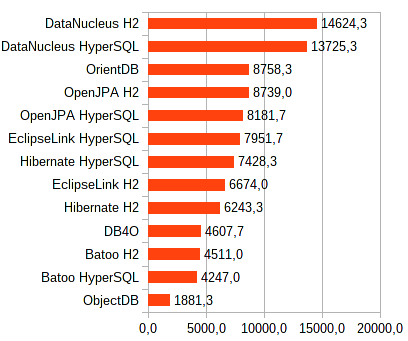
\includegraphics[]{obr/bench/resultf}
  \caption{Generování stromové struktury [ms]}\label{img:resultf}
\end{figure}
